\documentclass{article}
\usepackage{geometry}
\usepackage[T1]{fontenc}
\usepackage[utf8]{inputenc}
\usepackage{amssymb}
\usepackage{amsmath}
\usepackage{german}
\usepackage{tikz}
\usepackage{fancybox}

\geometry{a4paper, left=40mm, right=30mm, top=30mm, bottom=30mm}

\begin{document}
	\title{IPI Aufgabenblatt 2}
	
	\author{Benjamin Raach, Christoph Blattgerste\\ 
		\and Tutor: Enes Witwit}
	
	\maketitle
	
	\section*{Aufgabe 1}
	
	
	\section*{Aufgabe 2 a$)$}
	
	Infix Schreibweise:
	$\sqrt{(x*x) + (y*y) + (z*z)}$
	\newline
	
	Präfix Schreibweise
	$sqrt(add(mul(x,x), mul(y,y), mul(z,z)))$
	\newline
	
	Baumdiagramm:
	
	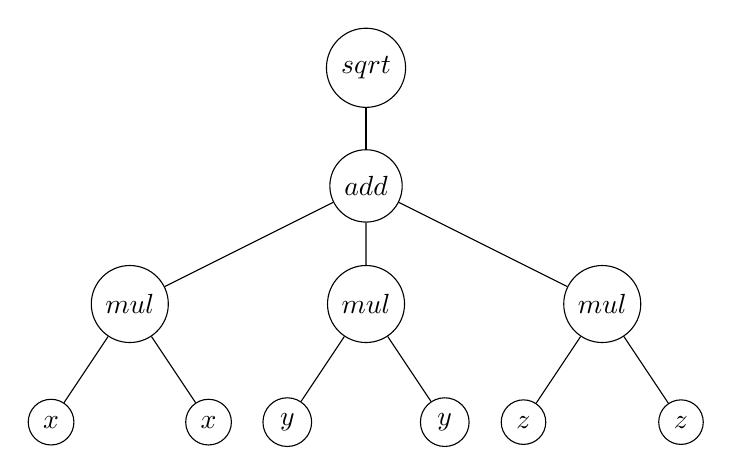
\begin{tikzpicture}[level/.style={sibling distance=60mm/#1}]
	
	\node [circle, draw] (z)  {$sqrt$}
		child {node [circle, draw] {$add$}
			child {node [circle, draw] {$mul$}
				child{node [circle, draw] {$x$}}
				child{node [circle, draw] {$x$}}
			}
			child {node [circle, draw] {$mul$}
				child{node [circle, draw] {$y$}}
				child{node [circle, draw] {$y$}}
			}
			child {node [circle, draw] {$mul$}
				child{node [circle, draw] {$z$}}			
				child{node [circle, draw] {$z$}}
			}
		};
	\end{tikzpicture}
	
	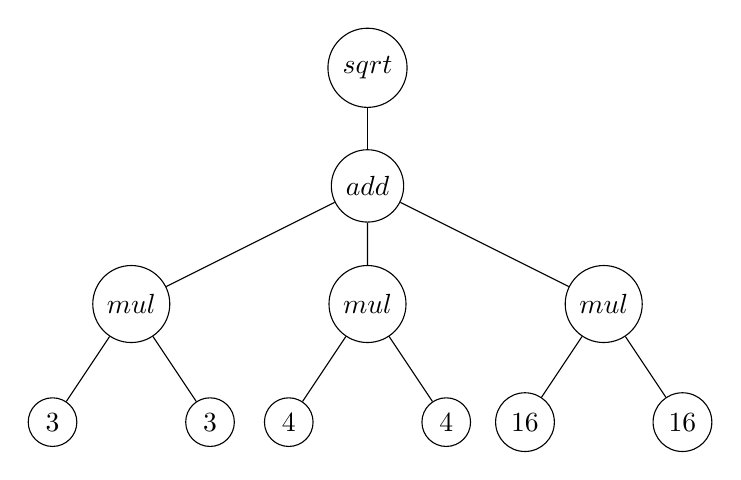
\begin{tikzpicture}[level/.style={sibling distance=60mm/#1}]
	
	\node [circle, draw] (z)  {$sqrt$}
	child {node [circle, draw] {$add$}
		child {node [circle, draw] {$mul$}
			child{node [circle, draw] {$3$}}
			child{node [circle, draw] {$3$}}
		}
		child {node [circle, draw] {$mul$}
			child{node [circle, draw] {$4$}}
			child{node [circle, draw] {$4$}}
		}
		child {node [circle, draw] {$mul$}
			child{node [circle, draw] {$16$}}			
			child{node [circle, draw] {$16$}}
		}
	};
	\end{tikzpicture}

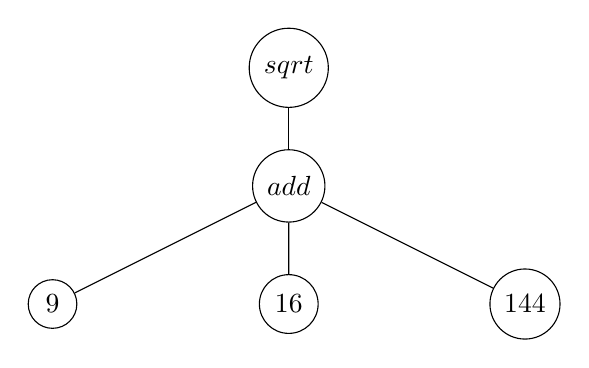
\begin{tikzpicture}[level/.style={sibling distance=60mm/#1}]

\node [circle, draw] (z)  {$sqrt$}
child {node [circle, draw] {$add$}
	child {node [circle, draw] {$9$}
	}
	child {node [circle, draw] {$16$}
	}
	child {node [circle, draw] {$144$}
	}
};
\end{tikzpicture}
	
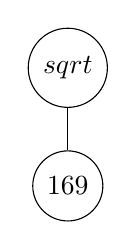
\begin{tikzpicture}[level/.style={sibling distance=60mm/#1}]

\node [circle, draw] (z)  {$sqrt$}
child {node [circle, draw] {$169$}
};
\end{tikzpicture}

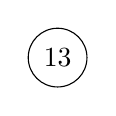
\begin{tikzpicture}[level/.style={sibling distance=60mm/#1}]

\node [circle, draw] (z)  {$13$};
\end{tikzpicture}
	
	\section*{Aufgabe 2 b$)$}
	Maschinensprache:
	
	\begin{align}
		&1 \quad 6 \quad 3 \\
		&1 \quad 7 \quad 4 \\
	 	&1 \quad 8 \quad 12 \\
	 	&4 \quad 5 \quad 8 \quad 8 \\
	  	&4 \quad 4 \quad 7 \quad 7 \\
	 	&4 \quad 3 \quad 6 \quad 6 \\
	 	&2 \quad 2 \quad 3 \quad 4 \quad 5 \\
	 	&6 \quad 1 \quad 2
	\end{align}
	
	\section*{Aufgabe 2 c$)$}
	Infix Ausdruck: \\
	$ (((2 + (3*x)) - (4*x*x)) + (5*x*x*x)) $ \\ \\
	
	Präfix Schreibweise: \\
	$add(sub((add(2, mul(3, x))), mul(4, x, x)), mul(5, x, x, x))$ \\ \\
	
	Baumdiagramm:
	
	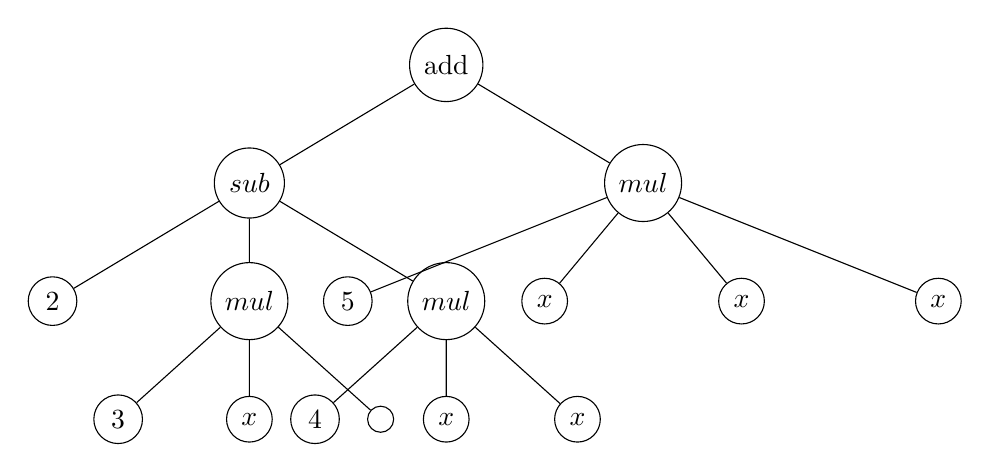
\begin{tikzpicture} [level/.style={sibling distance=50mm/#1}]
	\node [circle, draw] {add}
			child {node [circle, draw] {$sub$}
		child {node [circle, draw] {$2$}}
			child {node [circle, draw] {$mul$}
				child {node [circle, draw] {$3$}}
				child {node [circle, draw] {$x$}}
						child {node [circle, draw] {}}
			}
			child {node [circle, draw] {$mul$}
				child {node [circle, draw] {$4$}}
				child {node [circle, draw] {$x$}}
				child {node [circle, draw] {$x$}}
			}
		}
			child {node [circle, draw] {$mul$}
				child {node [circle, draw] {$5$}}
				child {node [circle, draw] {$x$}}
				child {node [circle, draw] {$x$}}
				child {node [circle, draw] {$x$}}
			}
	;\end{tikzpicture}
	
	\paragraph*{}
	
	Berechnung nach Substitutionsmodell:
	\begin{align}
	&\, add(sub(add(2, mul(3,2)), mul(4,2, 2)), mul(5, 2, 2, 2)) \\
	= &\, add(sub(add(2, 6), mul(4,2, 2)), mul(5, 2, 2, 2)) \\
	= &\, add(sub(8, 16), mul(5, 2, 2, 2)) \\
	= &\, add(-8, 40) \\
	= &\, 32
	\end{align}
	
	\section*{Aufgabe 2 d$)$}
	
	\begin{align}
		& \, 2 + (3 + (-4 + 5* x) * x) * x  \\
		= & \, 2 + (3 + ((-4 * x) + 5 * x * x) * x)  \\
		= & \, 2 + (3 + (-4 * x * x) + (5 * x * x * x)) \\
		= & \, 2 + (3 * x) + (-4 * x * x) + (5 * x * x * x)  \\
		= & \, 2 + (3 * x) - (4 * x * x) + (5 * x * x * x) \\
		= & \, add(2, sub(mul(3,x), mul(4, x, x)), mul(5, x, x, x)) \\
		= & \, add(sub(add(2, mul(3, x))), mul(4, x, x)), mul(5, x, x, x))
	\end{align}
	
	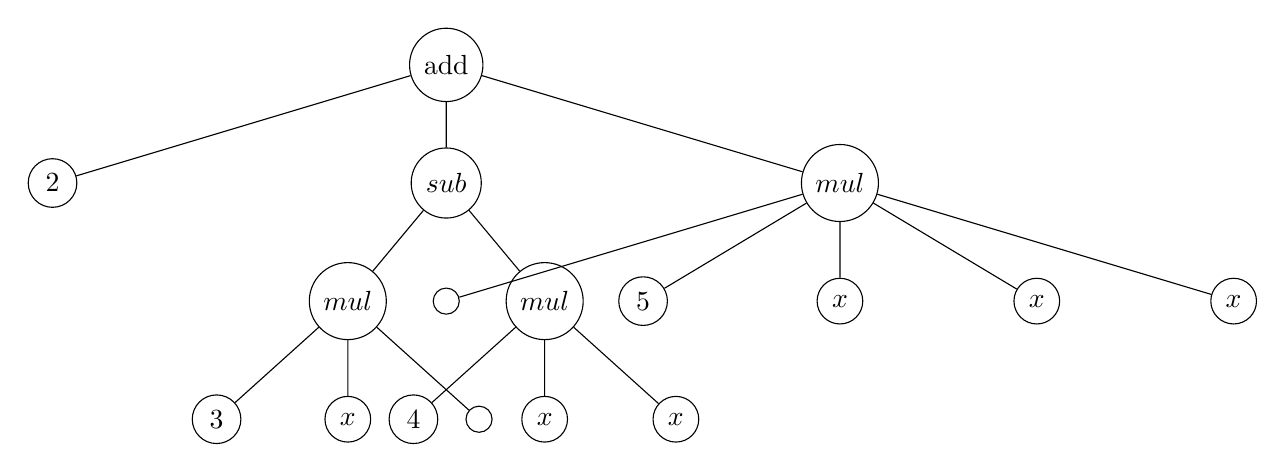
\begin{tikzpicture} [level/.style={sibling distance=50mm/#1}]
	\node [circle, draw] {add}
		child {node [circle, draw] {$2$}}
		child {node [circle, draw] {$sub$}
		child {node [circle, draw] {$mul$}
			child {node [circle, draw] {$3$}}
			child {node [circle, draw] {$x$}}
			child {node [circle, draw] {}}
		}
		child {node [circle, draw] {$mul$}
			child {node [circle, draw] {$4$}}
			child {node [circle, draw] {$x$}}
			child {node [circle, draw] {$x$}}
		}
	}
	child {node [circle, draw] {$mul$}
		child {node [circle, draw] {}}
		child {node [circle, draw] {$5$}}
		child {node [circle, draw] {$x$}}
		child {node [circle, draw] {$x$}}
		child {node [circle, draw] {$x$}}
	}
	;\end{tikzpicture}
	
	\begin{align}
			& \, add(2, sub(mul(3,2), mul(4, 2, 2)), mul(5, 2, 2, 2)) \\
			= & \, add(2, sub(6, 16), mul(5, 2, 2, 2)) \\
			= & \, add(2, -10, 40) \\
			= & \, 32
	\end{align}
	
	\section*{Aufgabe 2 e$)$}
	
	Maschinenprogramm:
	
	\begin{align}
	& 1 \quad 1 \quad 2 \\
	& 1 \quad 2 \quad 2 \\
	& 1 \quad 3 \quad 3 \\
	& 1 \quad 4 \quad 4 \\
	& 1 \quad 5 \quad 5 \\
	& 4 \quad 6 \quad 3 \quad 2 \\
	& 4 \quad 7 \quad 4 \quad 2 \\
	& 4 \quad 8 \quad 7 \quad 2 \\
	& 4 \quad 9 \quad 5 \quad 2 \\
	& 4 \quad 10 \quad 9 \quad 2 \\
	& 4 \quad 11 \quad 10 \quad 2 \\
	& 2 \quad 12 \quad 1 \quad 6  \\
	& 2 \quad 13 \quad 12 \quad 11 \\
	& 3 \quad 14 \quad 13 \quad 8 \\
	\end{align}
	
	\section*{Aufgabe 3}

			
	
\end{document}
